\title{%
  A Science of Security Course: Introduction
}
\author{Daniel Bosk\thanks{%
    This material was authored by Daniel Bosk and is available under the 
    Creative Commons Attribution-ShareAlike (CC-BY-SA) 4.0 international 
    license.
}}
\institute{%
  KTH EECS, \email{dbosk@kth.se}
}

\begin{pycode}
from mentipy.latex import mc, open_text
from mentipy.store import Store

mentipy_common = {
    "store": Store("mentipy.json"),
    "qr_dir": "mentipy-obj",
    "qr_format": "png",
    "environment": "exercise",
    "show_url": False,
    "layout": "auto",
    # The public poll address (mentipy serve --public ssh), not the LAN one
    "base_url": "http://faculty-shell.sys.kth.se:8080",
}
\end{pycode}
% Let the poll address under the QR code break to fit its column
\newcommand{\mentipyqrcaption}[1]{{\tiny\url{#1}}}

\mode<article>{\maketitle}
\mode<presentation>{%
  \begin{frame}
    \maketitle
  \end{frame}
}

\mode*

\begin{abstract}
  \emph{Summary:}
The course highlights, how different parts of the scientific methodology are 
relevant for cybersecurity in different situations. The focus is to analyse how 
scientific methods influence our knowledge of issues in cybersecurity, 
including their relation to different aspects of the subjects
\begin{itemize}
  \item gender equality, diversity and equal conditions
  \item sustainability,
  \item ethical dilemmas.
\end{itemize}

\emph{Intended learning outcomes:}
After passing the course, the student should be able to
\begin{itemize}
  \item \emph{relate} the different parts of scientific method, how they relate 
    to one another, contribute and not contribute to scientificity in security;
  \item \emph{assess, analyse, and discuss} the quality in, and ethical aspects 
    of, knowledge generation related to digital systems and in particular the 
    security of these systems;
  \item \emph{apply} scientific methodology to show how to answer issues in the 
    cybersecurity field;
  \item \emph{plan and carry out} assignments within given time frames and 
    available resources;
  \item \emph{write} short, clear and \emph{arguing} texts based on \emph{own 
    analysis} as well as given material
\end{itemize}
in order to be able to contribute to scientifically based development.

\emph{Prerequisites:}
Knowledge and skills in cyber security, the student should be able to:
\begin{itemize}
  \item identify threats against confidentiality, integrity and availability in 
    digital systems
  \item explain basic terminology and concepts in computer security and use 
    them
  \item find and use documentation of security related problems and tools
  \item analyse simple program code and systems (based on given or self-made 
    system descriptions) to identify vulnerabilities and predict corresponding 
    threats
  \item select countermeasures against identified threats and argue for their 
    suitability
  \item compare countermeasures and evaluate their side effects,
  \item apply countermeasures present and explain their reasoning to others.
\end{itemize}

Knowledge of the role of the cybersecurity engineer in society, the student 
should be able to:
\begin{itemize}
  \item analyse and discuss how the use and development of digital systems and 
    in particular the security of these systems affect and are affected by 
    social, economic, environmental, work environmental and ethical 
    sustainability as well as diversity, gender equality and equal conditions
  \item review critically and reflect on both the set-up and implementation of 
    the education as well as their own study situation, their skills in 
    relation to the objective of the education and the future professional role 
    and their ability to identify their own need of additional knowledge
  \item plan and carry out assignments within given time frames and using 
    available resources
  \item write short, clear and arguing texts based on own analysis as well as 
    given material.
\end{itemize}

Knowledge of scientific methodology, the student should, with regards to the 
theory and  methodology of science, both orally as well as in writing, be able 
to:
\begin{itemize}
  \item identify definitions and descriptions of concepts, theories and problem 
    areas, as well as identify the correct application of these concepts and 
    theories;
  \item account for concepts, theories and general problem areas, as well as 
    apply concepts and theories to specific cases;
  \item critically discuss the definitions and applications of concepts and 
    theories as they applies to specific cases of scientific research.
\end{itemize}

% XXX Assessment
\emph{Assessment:}
The intended learning outcomes are assessed in the form of written assignments 
(asynchronous) and active seminar participation (synchronous).

\end{abstract}

\clearpage
\tableofcontents
\clearpage

\section{Overview}

Let's have a look at provable security, widely considered the epitome of 
security research.

\begin{frame}
  \begin{example}[\enquote{Provable security}]\label{SecurePassword}
    A uniformly random string of length \(n\) is secure to use as a password.
    We can prove it will take millions of years to guess it.
  \end{example}

  \pause

  \begin{example}[Pentesting]
    Pentesters can still guess passwords and get in.
  \end{example}

  \pause

  \begin{remark}
    Neither informs us of what to do about it.
  \end{remark}
\end{frame}

\begin{frame}<presentation>
  \begin{example}[Usability]
    \begin{itemize}
      \item Turns out people can't handle uniformly random passwords.
      \item Particularly not with a unique such password for every service.
      \item They can't generate uniformly random passwords either.
    \end{itemize}
  \end{example}

  \pause

  \begin{remark}[Several aspects]
    \begin{itemize}
      \item We want students to handle complex problems.
      \item Should see there are several aspects.
      \item Aspects must be approached differently.
    \end{itemize}
  \end{remark}
\end{frame}

So, attackers still get in.
% XXX add refs to password literature
It turns out that humans can't handle long, uniformly random passwords.
Particularly not when they have to remember one such password \emph{per service 
they use}.
And they can't generate uniformly random passwords either!
None of these results could be found through provable security, they're from 
the usability area of security and the methods are from the usability and 
human--computer interaction research field.

By this we don't say that provable security is wrong or doesn't work.
The same can be said of the usability methods.
Both are needed, they complement each other in generating understanding of 
security problems.
The goal of the course is that the students should be able to master the 
variety of methods and combine them to answer questions about security 
problems.
That includes being able to evaluate different approaches to answering 
questions and choosing among the most suitable ones.

\only<presentation>{\subsection{The goal}}

The goal of the course is to give a holistic view of the Science of Security.
We want to answer the following question:

\begin{frame}
  \begin{question}
    What are the \emph{research} methods we (in the security community) use and 
    why?
  \end{question}
\end{frame}

\begin{frame}<presentation>
  \begin{block}{The goal}
    \begin{itemize}
      \item Give a holistic view of \emph{Science} of Security.
    \end{itemize}
  \end{block}
\end{frame}

This is a tricky question to answer, because there are some apparent problems 
with the scientificity in the security area.
Consider the following examples.

\begin{frame}[fragile]
  \begin{example}\label{SoKProblem1}
      \textcquote[\S IV]{SecurityAsAScience}{%
        \textins*{C}laims of necessary conditions for real-world security are 
        unfalsifiable.
        Claims of necessary conditions for formally-defined security are 
        tautological restatements of the assumptions.%
      }
  \end{example}

  \pause

  \begin{example}\label{SoKProblem2}
    \textcquote{SecurityAsAScience}{%
      Unfalsifiable claims are common in security---and they, along with 
      circular arguments, are used to justify many defensive measures 
      \textelp{}
      \textins{T}here are many ways to argue measures in, but no way to argue 
      one out.%
    }
  \end{example}
\end{frame}

Before we look at what makes such claims unfalsifiable, try the following
exercise on six claims: \enquote{all swans are white}, \enquote{there are no
UFOs}, \enquote{UFOs exist}, \enquote{this system is secure}, \enquote{this
system is insecure} and the password rule \enquote{to be secure, a password
must have at least 8 characters and contain letters, digits and special
characters}.

\begin{frame}[fragile]
  \begin{pycode}
print(mc(
    "Which of these claims could a single observation show to be false?",
    [
        "All swans are white.",
        "There are no UFOs.",
        "UFOs exist.",
        "This system is secure.",
        "This system is insecure.",
        "To be secure, a password must have at least 8 characters and "
        "contain letters, digits and special characters.",
    ],
    multi=True,
    **mentipy_common,
))
  \end{pycode}
\end{frame}

\ltnote{%
  Asked before the asymmetry is explained, so that the answers show whether
  students already separate claims an observation can refute from claims it
  can only confirm.
  The options vary the form of the claim (universal, non-existence,
  existence) and pair each everyday claim with a security claim of the same
  form.
  Each wrong answer marks one misconception: choosing \enquote{UFOs exist} or
  \enquote{This system is insecure} confuses confirming a claim with refuting
  it; missing \enquote{There are no UFOs} or \enquote{This system is secure}
  takes negative or security claims to be untestable; choosing the password
  rule takes a prescription to be testable as stated.
  The UFO pair comes from the author's own note in the margin of
  \citeauthor{SecurityAsAScience}'s Section~II-B.%
}

A black swan refutes \enquote{all swans are white} and a UFO refutes
\enquote{there are no UFOs}, but no observation refutes \enquote{UFOs exist}:
not having seen one only means that we haven't looked in the right place.
It is the other way around for confirmation: one UFO confirms that UFOs exist,
but no number of white swans confirms that all swans are white.
Security claims have the same asymmetry (\cref{tab:refute-confirm}).

\begin{frame}
  \begin{table}
    \footnotesize
    \begin{tabular}{lll}
      \toprule
      Claim & Refuted by & Confirmed by \\
      \midrule
      All swans are white. & a black swan & nothing \\
      There are no UFOs. & a UFO & nothing \\
      UFOs exist. & nothing & a UFO \\
      This system is secure. & a successful attack & nothing \\
      This system is insecure. & nothing & a successful attack \\
      The password rule. & nothing & nothing \\
      \bottomrule
    \end{tabular}
    \caption{What a single observation can do to each claim: a claim that
      something holds everywhere can be refuted but not confirmed, a claim
      that something exists can be confirmed but not refuted.}
    \label{tab:refute-confirm}
  \end{table}
\end{frame}

\Textcite{SecurityAsAScience} put it as follows, and use the password rule as
their example.

\begin{frame}
  \begin{example}
    \textcquote[p.~109]{SecurityAsAScience}{%
      We can observe that something is insecure (by observing a failure) but
      no observation allows us to determine empirically that something is
      secure\textelp{}%
    }
  \end{example}

  \pause

  \begin{example}
    \textcquote[p.~110]{SecurityAsAScience}{%
      To falsify the claim \enquote{a password must have at least 8
      characters and contain letters, digits and special characters to be
      secure} we would have to find a secure non-compliant password.
      However, we can't find a secure password, since successfully avoiding
      harm in the past is no guarantee about the future.%
    }
  \end{example}
\end{frame}

So the rule as stated cannot be tested.
Can it be turned into a claim that can?

\begin{frame}[fragile]
  \begin{pycode}
print(open_text(
    "Rewrite the password rule from the previous slide so that an "
    "observation could show it to be false.",
    max_chars=280,
    next=False,
    **mentipy_common,
))
  \end{pycode}
\end{frame}

One way is to turn the rule into a prediction about outcomes, which an
observation can contradict.
That prediction has been tested, but late, since
\textcquote[p.~110]{SecurityAsAScience}{%
  storing passwords as salted hashes \textelp{} precluded easily measuring
  whether mandates on character composition were having the predicted
  effect.
  Recent empirical work shows that they do not%
}.

\begin{frame}
  \begin{block}{A version that can be refuted}
    Accounts whose passwords follow the rule are guessed less often than
    accounts whose passwords don't.
  \end{block}

  \pause

  \begin{remark}
    \textcquote[p.~101]{SecurityAsAScience}{%
      Stating the evidence that would falsify a claim thus acts as a forcing
      function to clarify vague claims and implicit assumptions.%
    }
  \end{remark}
\end{frame}

This leads us to the second question, we want the students to able to answer:

\begin{frame}
  \begin{question}
    What makes my work (in security) scientific?
  \end{question}
\end{frame}

\begin{frame}<presentation>
  \begin{block}{Aim of Science of Security course}
    \begin{itemize}
      \item Complement the general methods course (TAMOS).
      \item Better prepare students for thesis (and hopefully worklife \dots).
      \item They should be able to contribute to \emph{scientifically} based 
        development in cybersecurity.
    \end{itemize}
  \end{block}

  \begin{remark}
    \begin{itemize}
      \item This course is now fully synced with TAMOS\@.
    \end{itemize}
  \end{remark}
\end{frame}

\only<article>{\subsection{Goals and requirements}}

Now the aim of the course is to complement the general scientific methods 
course.
Due to the complexity of security problems and the field's interdisciplinary 
composition, we want to emphasise on how the methods fit together in the field.
We find this particularly necessary after reading the quotes in 
\cref{SoKProblem1,SoKProblem2}.

The requirements for Master's level are set out in 
\citetitle{HEO2}~\autocite{HEO2}, namely:
%\begin{frame}[fragile]
  \begin{block}{Master's goals: Knowledge and understanding~\autocite{HEO2}}
    \only<article>{\begin{enumerate}[label={(K\arabic*)},ref=K\arabic*]}
    \only<presentation>{\begin{itemize}}
      \item\label{K1} demonstrate knowledge and understanding \textelp{} as 
        well as insight into current research and development work, and
      \item\label{K2} demonstrate specialised methodological knowledge in the 
        main field of study.
      \item\label{K3} demonstrate the ability to critically and systematically 
        integrate knowledge and analyse, assess and deal with complex 
        phenomena, issues and situations even with limited information
    \only<article>{\end{enumerate}}
    \only<presentation>{\end{itemize}}
  \end{block}
%\end{frame}

%\begin{frame}[fragile]
  \begin{block}{Master's goals: Competence and skills~\autocite{HEO2}}
    \only<article>{\begin{enumerate}[label={(C\arabic*)},ref=C\arabic*]}
    \only<presentation>{\begin{itemize}}
      \item\label{C1} demonstrate the ability to identify and formulate issues 
        critically, autonomously and creatively as well as to plan and, using 
        appropriate methods, undertake advanced tasks
        \only<presentation>{\textelp{}}%
        \only<article>{within predetermined time frames}
        and so contribute to the formation of knowledge as well as the ability 
        to evaluate this work
      \item\label{Ccomm} demonstrate the ability in speech and writing both 
        nationally and internationally to clearly report and discuss his or her 
        conclusions and the knowledge and arguments on which they are based in 
        dialogue with different audiences, and
      \item\label{C2} demonstrate the skills required for participation in 
        research and development work \textelp{}
    \only<presentation>{\end{itemize}}
    \only<article>{\end{enumerate}}
  \end{block}
%\end{frame}

%\begin{frame}[fragile]
  \begin{block}{Master's goals: Judgement and approach~\autocite{HEO2}}
    \only<article>{\begin{enumerate}[label={(J\arabic*)},ref=J\arabic*]}
    \only<presentation>{\begin{itemize}}
      \item\label{J1} demonstrate the ability to make assessments in the main 
        field of study informed by relevant disciplinary, social and ethical 
        issues and also to demonstrate awareness of ethical aspects of research 
        and development work
      \item\label{J2} demonstrate insight into the possibilities and 
        limitations of research, \textelp{}
    \only<presentation>{\end{itemize}}
    \only<article>{\end{enumerate}}
  \end{block}
%\end{frame}

\paragraph{Intended learning outcomes}\label{LearningOutcomes}

\begin{frame}[fragile]
  \only<article>{In summary, the learning outcomes, we want that after}%
  \only<presentation>{After}%
  passing the course, the student should be able to
  \only<article>{\begin{enumerate}[label={(LO\arabic*)},ref=LO\arabic*]}
  \only<presentation>{\begin{itemize}}
    \item\LOrelate*
      \only<article>{[\ref{K1}, \ref{K2}, \ref{J2}]}
    \item\LOevaluate*
      \only<article>{[\ref{C1}, \ref{C2}, \ref{J1}, \ref{K3}]}
    \item\LOapply*
      \only<article>{[\ref{C1}, \ref{C2}]}
    \only<presentation>{%
    \item \dots
    }
    \only<article>{%
    \item\LOplan*
      \only<article>{[\ref{C1}]}
    \item\LOcomm*
      \only<article>{[\ref{K3}, \ref{Ccomm}]}
    }
  \only<presentation>{\end{itemize}}
  \only<article>{\end{enumerate}}
  in order to be able to contribute to scientifically based development.
\end{frame}

There are also two learning outcomes related more to general skill, rather than 
scientific method:
\begin{frame}[fragile]
  After passing the course, the student should be able to
  \begin{itemize}
    \item plan and carry out assignments within given time frames and using 
      available resources, and
    \item write short, clear and arguing texts based on own analysis as well as 
      given material.
  \end{itemize}
\end{frame}

\subsection<article>{Prerequisites}

The course requires some prerequisites.
In the area of cybersecurity, the student should be able to:
\begin{itemize}
  \item identify threats against confidentiality, integrity and availability in 
    digital systems
  \item explain basic terminology and concepts in computer security and use 
    them
  \item find and use documentation of security related problems and tools
  \item analyse simple program code and systems (based on given or self-made 
    system descriptions) to identify vulnerabilities and predict corresponding 
    threats
  \item select countermeasures against identified threats and argue for their 
    suitability
  \item compare countermeasures and evaluate their side effects,
  \item apply countermeasures present and explain their reasoning to others.
\end{itemize}

In the area of the cybersecurity engineer's role in society, the student should 
be able to:
\begin{itemize}
  \item analyse and discuss how the use and development of digital systems and 
    in particular the security of these systems affect and are affected by 
    social, economic, environmental, work environmental and ethical 
    sustainability as well as diversity, gender equality and equal conditions
  \item review critically and reflect on both the set-up and implementation of 
    the education as well as their own study situation, their skills in 
    relation to the objective of the education and the future professional role 
    and their ability to identify their own need of additional knowledge
  \item plan and carry out assignments within given time frames and using 
    available resources
  \item write short, clear and arguing texts based on own analysis as well as 
    given material.
\end{itemize}

Finally, since course is intended to complement the general research methods 
course, we expect the students to, with regards to the theory and  methodology 
of science, both orally as well as in writing, be able to:
\begin{itemize}
  \item identify definitions and descriptions of concepts, theories and problem 
    areas, as well as identify the correct application of these concepts and 
    theories;
  \item account for concepts, theories and general problem areas, as well as 
    apply concepts and theories to specific cases;
  \item critically discuss the definitions and applications of concepts and 
    theories as they applies to specific cases of scientific research.
\end{itemize}


\section{More concretely}

Let's return to the goal of the course and then proceed to its contents.

\subsection{The goal}

The goal of the course is that the students should be able to master the 
variety of methods [\ref{LOrelate}] and combine them to answer questions about 
security problems [\ref{LOapply}].
That includes being able to evaluate different approaches to answering 
questions and choosing among the most suitable ones [\ref{LOevaluate}].

Knowledge dissemination is about communicating results to others.
And in science, to convince others that one's results are correct.
We can see this aspect in \ref{LOcomm} (and \ref{Ccomm}) and we will see this 
aspect as part of the assessment of the course later.

\begin{frame}
  \begin{block}{Concrete goals}
    \begin{itemize}
      \item Ask good questions.
      \item Propose suitable methods to answer them.
      \item Evaluate the suitability of proposed methods.
    \end{itemize}
  \end{block}

  \begin{remark}
    \begin{itemize}
      \item The focus is on \emph{research methods}.
      \item It's \emph{not} on {constructing a secure solution}.
      \item We want to know \emph{how do you know if it is secure?}
    \end{itemize}
  \end{remark}
\end{frame}


\subsection{Format}

We have the following division of credits in LADOK\footnote{%
  See the syllabus:
  \url{https://www.kth.se/student/kurser/kurs/DA2215?l=en}.
}\footnote{%
  There is a similar line in DD2302.
}:
\begin{description}
  \item[INL1] Seminars and assignments, 3.0 credits, grading scale: P, F
\end{description}

The assignments consists of reading and social annotation in an online tool 
(\cref{fbfdocquiz,fbfdocannotation}).
All seminars are live in the class Zoom room; only this introduction is also
on campus (D37).
You pass the course either by taking part in all teaching or by doing a final
project; the final seminar is only for those who do the project.

\begin{figure*}[t]
  \begin{sidecaption}
    {Two ways of having interactive documents.}
    [fbfdoc]
    \begin{subfigure}[b]{0.49\columnwidth}
      \centering
      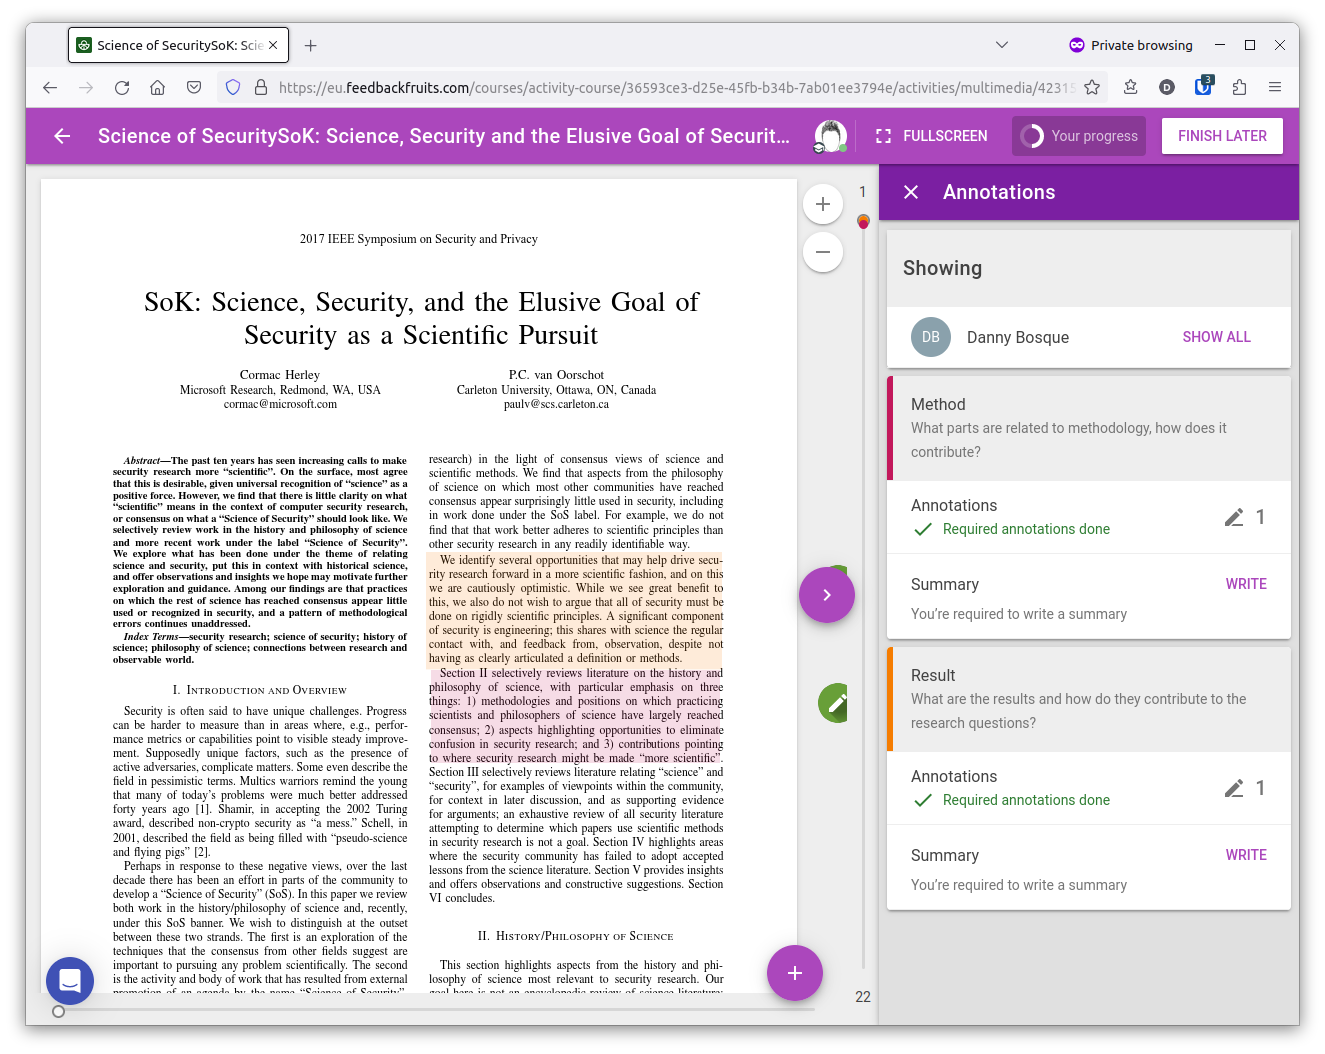
\includegraphics[width=\columnwidth]{figs/fbf-doc-annotations.png}
      \caption{%
        An interactive document in FeedbackFruits where one can annotate the 
        text with focused topics together with other students in the class.%
        \label{fbfdocannotation}%
      }
    \end{subfigure}
    \hfill
    \begin{subfigure}[b]{0.49\columnwidth}
      \centering
      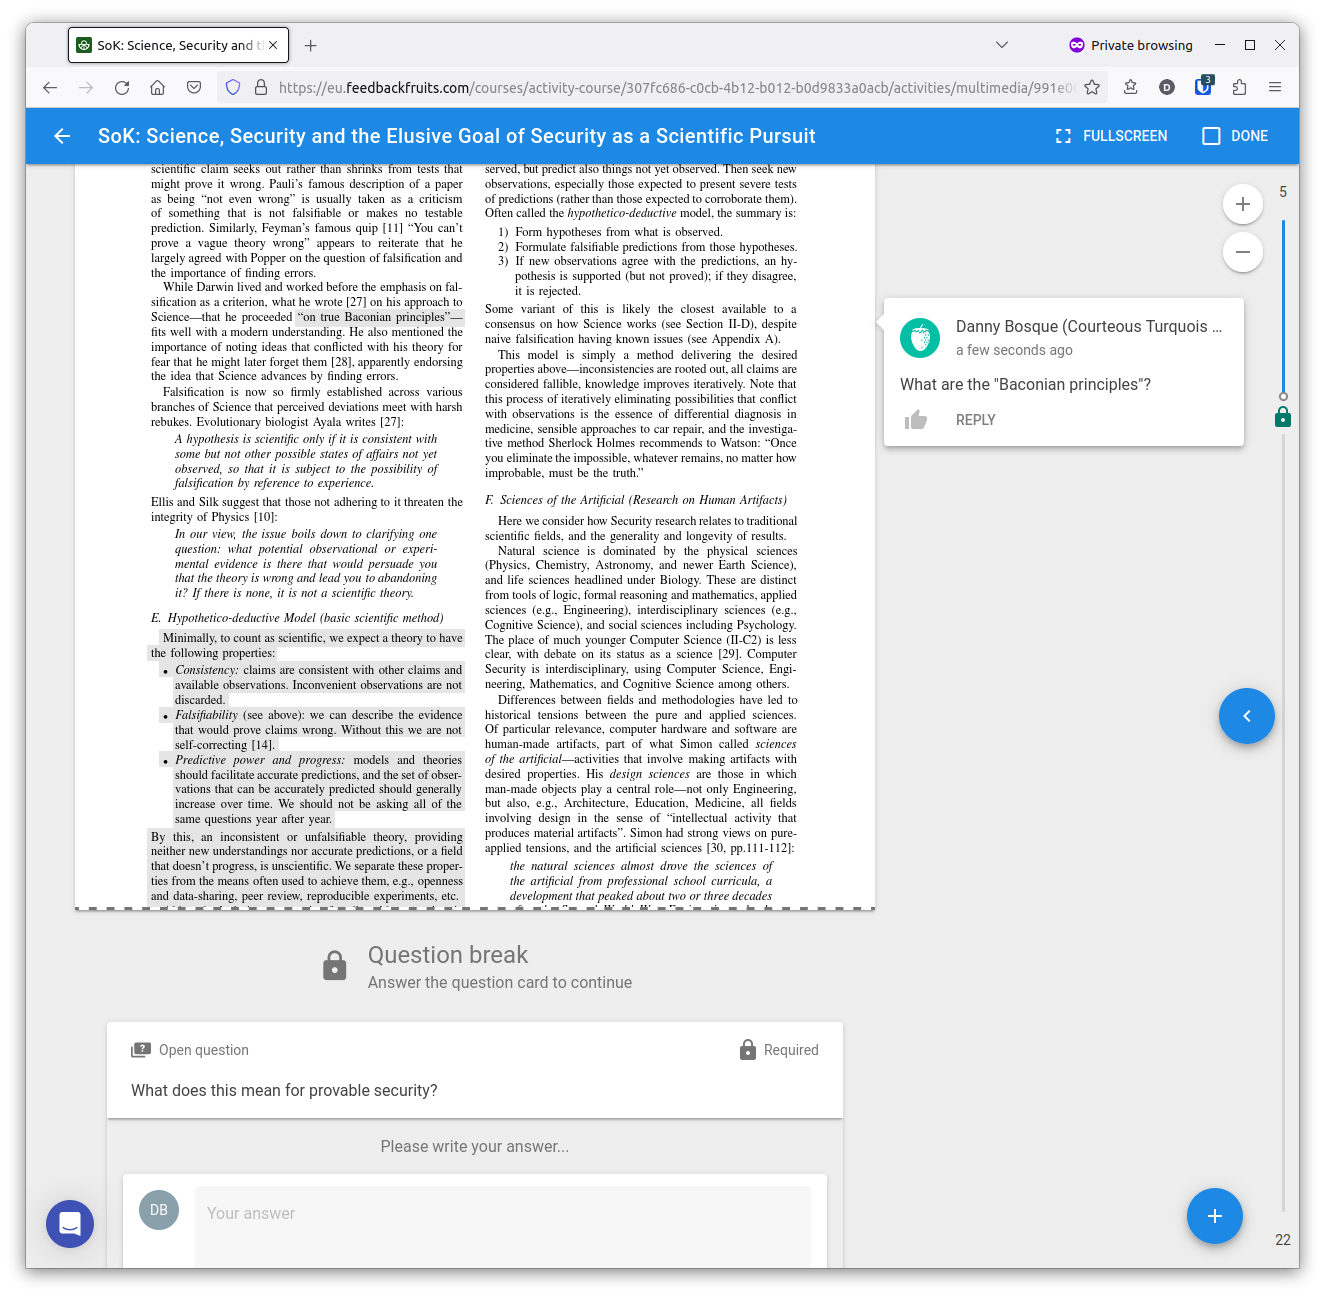
\includegraphics[width=\columnwidth]{figs/fbf-doc-quiz-question.png}
      \caption{%
        An interactive document in FeedbackFruits where one can answer quiz 
        questions posed in the document and ask questions about the content.%
        \label{fbfdocquiz}%
      }
    \end{subfigure}
  \end{sidecaption}
\end{figure*}

\mode<presentation>{%
\begin{frame}
  \begin{block}{Examination}
    \begin{description}
      \item[INL1] Seminars and assignments, 3.0 credits, grading scale: P, F
    \end{description}
  \end{block}

  \pause

  \begin{block}{Format}
    \begin{itemize}
      \item Online prep: FeedbackFruits and reflections
      \item Live seminars online, in the class Zoom room
      \item Final seminar (project) online: Mon 4/1 08:15 or Tue 5/1 13:15
    \end{itemize}
  \end{block}
\end{frame}
}

The reading assignments are part of the learning material.
These are complemented by interactive video lectures (\cref{fbfvideo}) and the
live seminars.
In the video lectures the students can ask questions and answer quizzes.
The live seminars aim at exploring the paths not taken in the material.

\begin{marginfigure}
  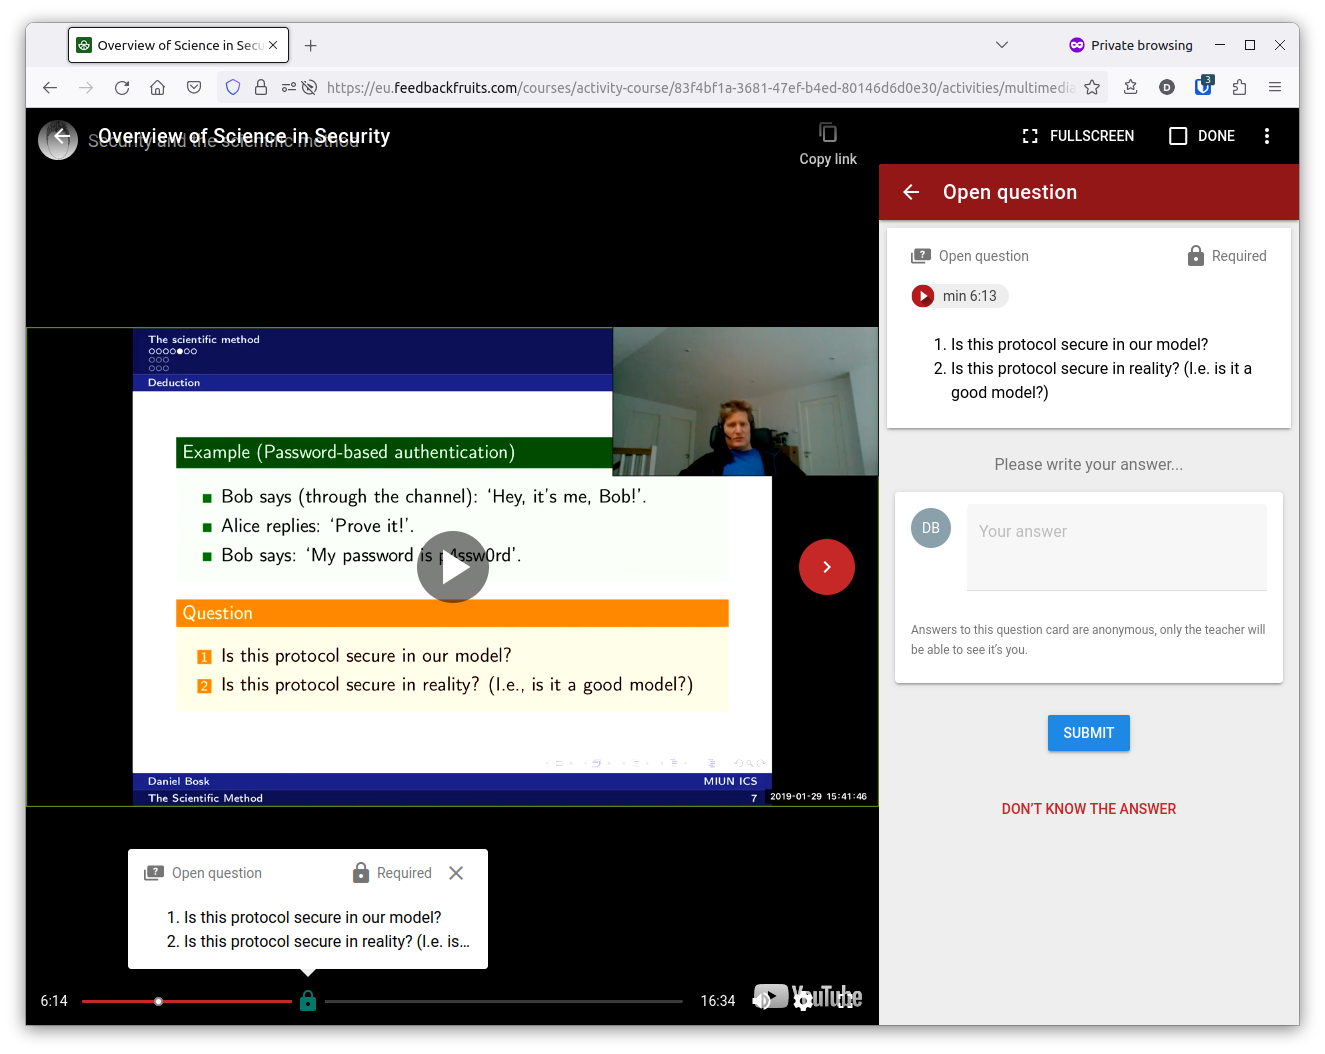
\includegraphics[width=\columnwidth]{figs/fbf-video-quiz.png}
  \caption{%
    An interactive video in FeedbackFruits where one can answer quiz 
    questions posed in the video.%
  }\label{fbfvideo}
\end{marginfigure}


\mode<presentation>{%
\begin{frame}
  \begin{columns}
    \begin{column}{0.5\columnwidth}
      \begin{block}{Teaching material}
        \begin{itemize}
          \item<1> Video lectures where students can ask questions and answer 
            quizzes.

          \item<2-3> Reading assignments with social annotation.
        \end{itemize}
      \end{block}
    \end{column}
    \begin{column}{0.5\columnwidth}
      \only<1>{
        \begin{figure}
          \centering
          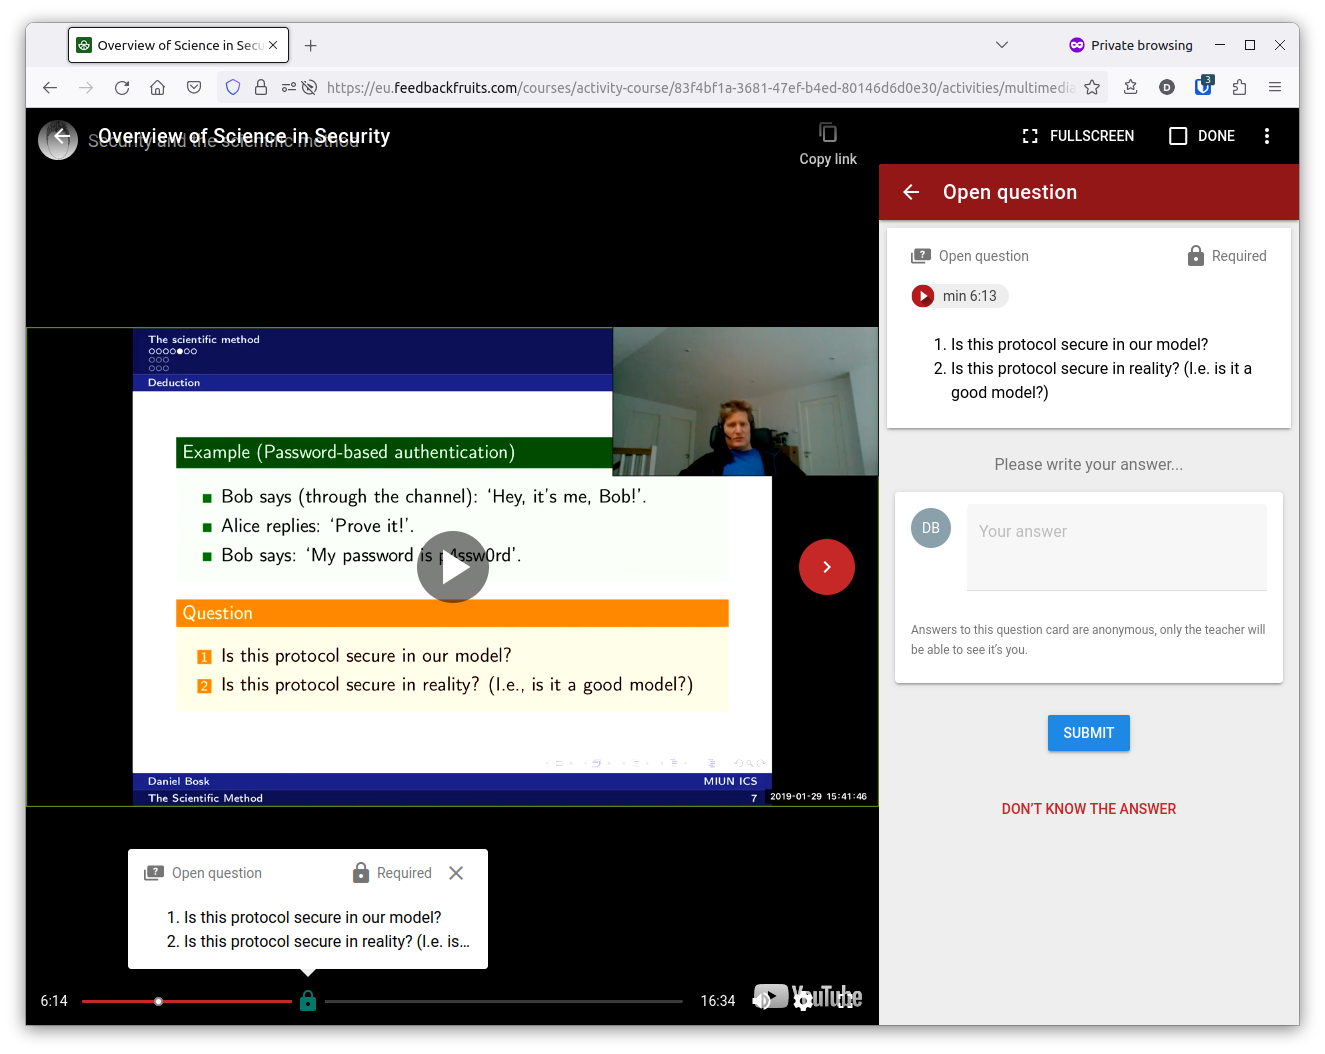
\includegraphics[width=\columnwidth]{figs/fbf-video-quiz.png}
          \caption{%
            An interactive video in FeedbackFruits where one can answer quiz 
            questions posed in the video.%
          }
        \end{figure}
      }
      \only<2>{
        \begin{figure}
          \centering
          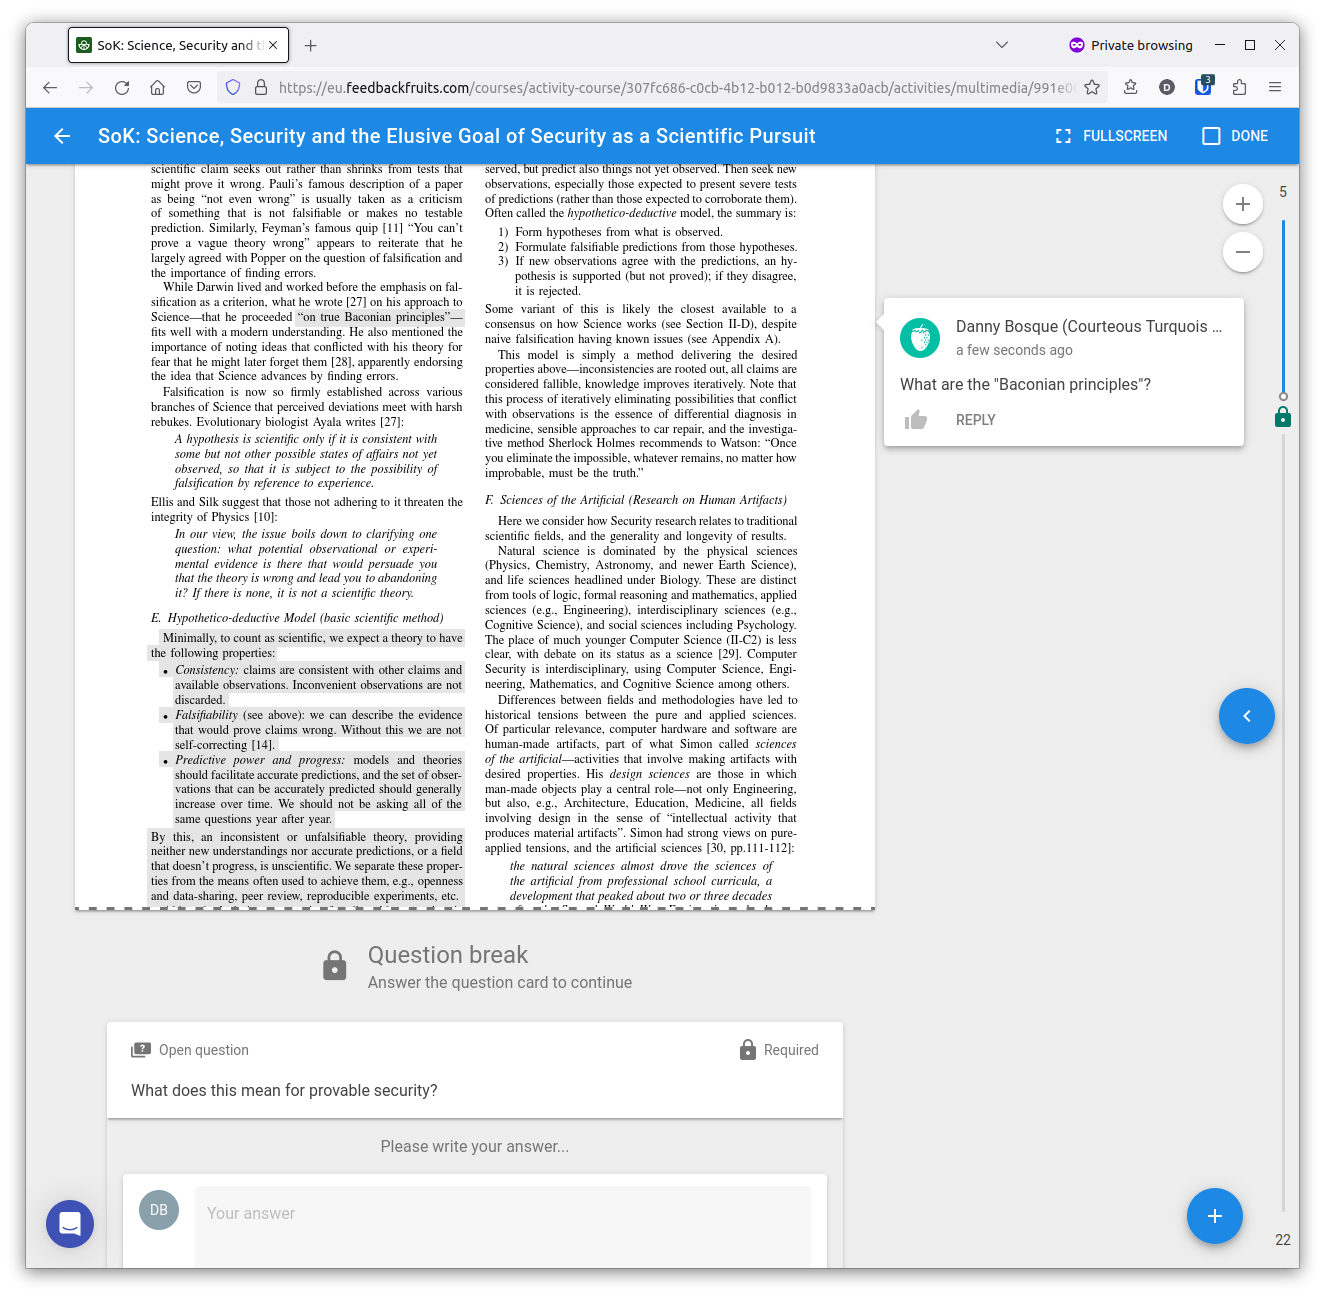
\includegraphics[width=\columnwidth]{figs/fbf-doc-quiz-question.png}
          \caption{%
            An interactive document in FeedbackFruits where one can answer quiz 
            questions posed in the document and ask questions about the 
            content.%
          }
        \end{figure}
      }
      \only<3>{
        \begin{figure}
          \centering
          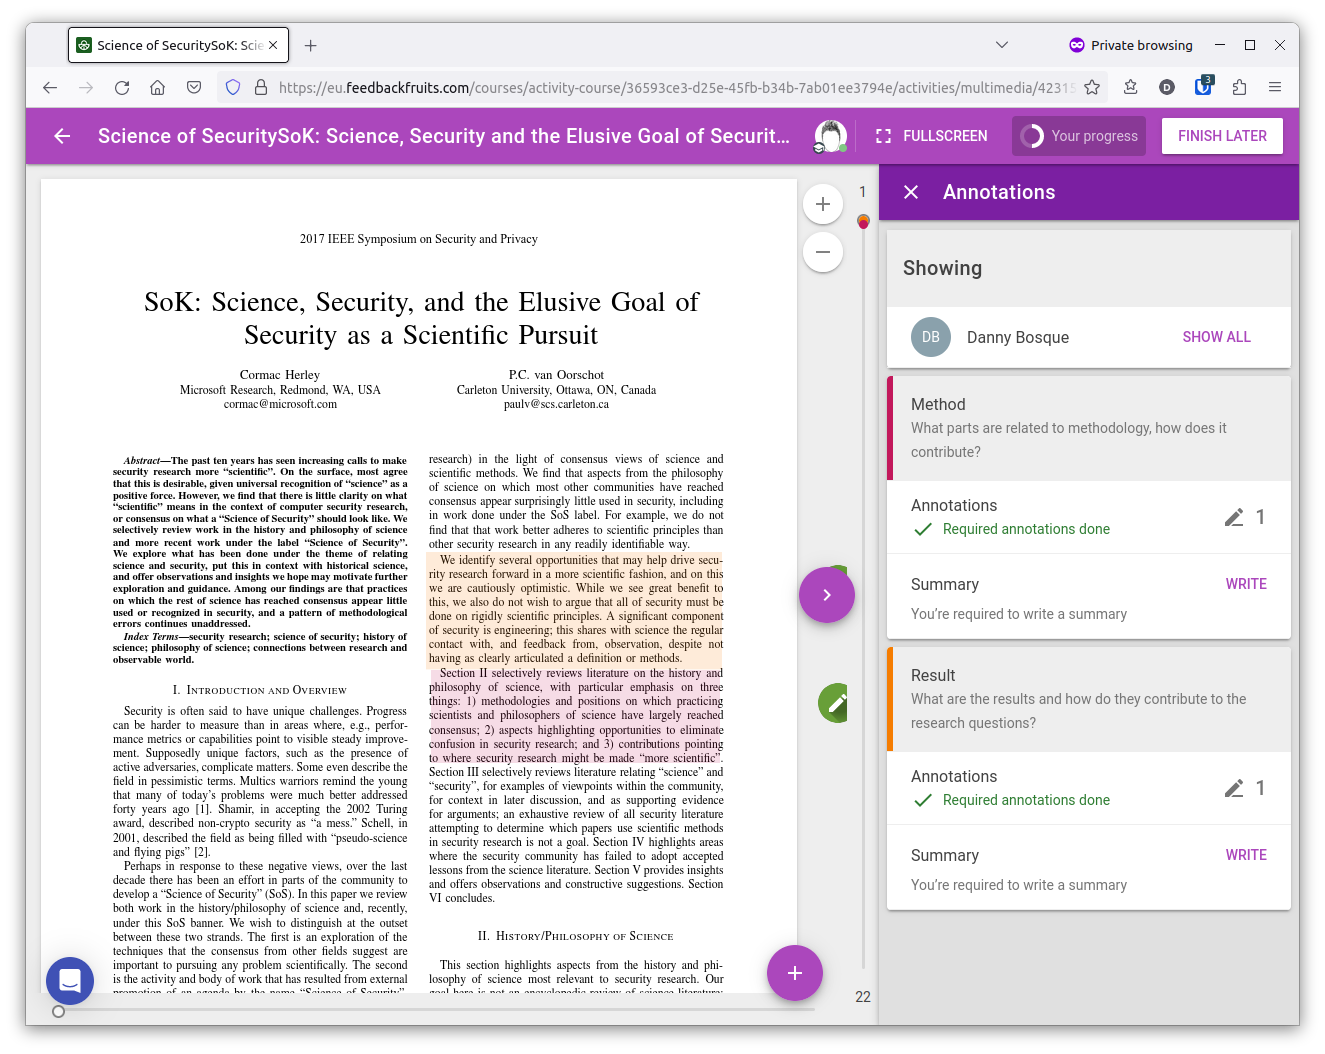
\includegraphics[width=\columnwidth]{figs/fbf-doc-annotations.png}
          \caption{%
            An interactive document in FeedbackFruits where one can annotate 
            the text with focused topics together with other students in the 
            class.%
          }
        \end{figure}
      }
    \end{column}
  \end{columns}
\end{frame}
}

The seminars are used as synchronization points.
Those who do the project also present it at a final seminar, which results in
their grade.

There are two independent ways to pass.
By participation: every FeedbackFruits assignment at 100/100 (not the TAMOS
videos), every reflection, both before the respective seminar, every live
seminar, and \enquote{Course evaluation survey (participation)}; that alone passes
the course, and opening the project assignments does no harm.
By project: the report, an individual review of another group's report (it is
fine to discuss it in the group), the final seminar, and \enquote{Course
evaluation survey (project)}.
Both surveys open on Monday 4/1, in the last week of the course, since the date
of the result must fall then (CSN).

\mode<presentation>{%
\begin{frame}
  \begin{block}{Teaching}<+>
    \begin{enumerate}
      \item Reading material and watching videos.
      \item Write reflection to prepare for seminar.
      \item Discuss and work with material at synchronous seminars.
    \end{enumerate}
  \end{block}

\end{frame}

\begin{frame}
  \begin{block}{Two ways to pass}
    \small
    \begin{description}
      \item[Participation] Every FeedbackFruits assignment at \alert{100/100}
        (not the TAMOS videos) and every reflection, before each seminar; every
        live seminar; \emph{Course evaluation survey (participation)}.
        That alone passes the course.
      \item[Project] Report, an individual review of another group's report,
        the final seminar; \emph{Course evaluation survey (project)}.
    \end{description}
  \end{block}

  \begin{remark}
    Both surveys open Mon 4/1, the last week of the course: the date of your
    result must fall then (CSN).
  \end{remark}
\end{frame}

\begin{frame}
  \begin{block}{Giving the course}
    \begin{itemize}
      \item Given twice per year: period 2 and 4.
      \item If you don't finish, you can try again next round.
    \end{itemize}
  \end{block}
\end{frame}
}

\Cref{tab:schedule} shows when the live seminars are and when their prep is
due.
All modules are open from the start; the week numbers in their names say when
to work on them.
The project has its deadlines before the final seminar: the draft report on
Sunday 20/12 and the peer review on Wednesday 30/12, both at 20:00.
The final version of the report is handed in after the seminar.

\begin{frame}
  \begin{table}
    \footnotesize
    \begin{adjustbox}{max width=\linewidth}
    \begin{tabular}{lll}
      \toprule
      Seminar & Topic & Prep due (20:00) \\
      \midrule
      Thu 12/11 09:15 & Literature reviews, with the library & Wed 11/11 \\
      Tue 17/11 08:15 & Inferences, experiments and measurements & Mon 16/11 \\
      Mon 23/11 08:15 & Models & Sun 22/11 \\
      Thu 3/12 13:15 & Quantitative and qualitative methods & Wed 2/12 \\
      Mon 7/12 08:15 & Science of security & Sun 6/12 \\
      4/1 08:15, 5/1 13:15 & Final seminar (project) & Draft: Sun 20/12 \\
      & & Review: Wed 30/12 \\
      \bottomrule
    \end{tabular}
    \end{adjustbox}
    \caption{The live seminars, all in the class Zoom room, and when their
      prep is due. The project instructions open on Monday 9/11; the
      final version of the report is handed in after the final seminar.}
    \label{tab:schedule}
  \end{table}
\end{frame}

Generative AI may be used as long as it follows the course guidelines, see the
page \enquote{How may AI be used in the course?} in the Course overview module.

\begin{frame}
  \begin{block}{Generative AI}
    \small
    \begin{description}
      \item[Allowed] Ideas, feedback on your text, the AI tools taught in the
        course, discussing the course content.
      \item[Not allowed] AI-written solutions, reports or reflections, or parts
        of them; asking AI to fix the feedback you got.
      \item[Always] Disclose your use. You must be able to do, explain and
        defend the work yourself.
    \end{description}
  \end{block}
  See \enquote{How may AI be used in the course?} in the Course overview
  module.
\end{frame}

\subsection{Contents}

The course starts with an overview of the complexity.
Then we proceed through a series of \enquote{How do you know it's secure?} case 
studies (assignments mentioned above), that are discussed in five live seminars
(\cref{tab:schedule}).
The idea is to explore how different research methods play together to answer 
different research questions.

\mode<presentation>{%
\begin{frame}
  \begin{block}{Contents}
    \begin{itemize}
      \item Overview of the complexity
    \end{itemize}
    \begin{enumerate}
      \item Purely deductive methods
      \item[\vdots]
      \item[n] Purely inductive methods
    \end{enumerate}
    \begin{itemize}
      \item {Philosophy of Science of Security}
    \end{itemize}
  \end{block}

  \pause

  \begin{remark}[What to focus]
    \begin{itemize}
      \item What do the various methods contribute?
      \item How do these play together? (Holistic view)
      %\item Emphasize the deduction/induction 
        %divide~\cite{SecurityAsAScience}.
    \end{itemize}
  \end{remark}
\end{frame}
}

We'll try to answer questions like
\enquote{What can deduction possibly say about reality?}
and \enquote{What can induction possibly say about security?}.
And what are the limitations?

\mode<presentation>{%
\begin{frame}
  \begin{example}[Deductive inquiry]
    \begin{itemize}
      \item \enquote{What can deduction possibly say about reality?}
    \end{itemize}
  \end{example}

  \pause

  \begin{example}[Inductive/empirical inquiry]
    \begin{itemize}
      \item \enquote{What can induction possibly say about security?}
    \end{itemize}
  \end{example}

  \pause

  \begin{remark}[To focus on]
    \begin{itemize}
      \item What are the limitations?
    \end{itemize}
  \end{remark}
\end{frame}
}

We'll end the teaching part with a seminar more towards the philosophy of 
science of security.
We'll depart in the paper 
\citetitle{SecurityAsAScience}\autocite{SecurityAsAScience} by
\citeauthor{SecurityAsAScience}.


\section{Contents}

%\begin{frame}
%  \begin{block}{Contents, part II}
%    \begin{itemize}
%      \item General introductions to various subfields.
%      \item Which methods are used and why?
%      %\item Some exemplary papers? \alert<2>{Both good and bad!}
%      \item How does a subfield fit into the holistic picture of Security?
%      \item How can these methods fit into other situations?
%    \end{itemize}
%  \end{block}
%
%  \begin{exercise}
%    \begin{itemize}
%      \item What is an area or problem that you're interested in (in security)?
%      \item Think of an interesting case that you can reflect on during the 
%        course.
%    \end{itemize}
%  \end{exercise}
%\end{frame}

%\begin{frame}
%  \begin{remark}
%    \begin{itemize}
%      \item All above was top down: faculty\footnote{%
%          From different subfields.
%        } present their view on
%        \begin{itemize}
%          \item the methodologies,
%          \item the practices,
%          \item the adversary models,
%          \item the assumptions,
%          \item the relation to scientific approach in their respective 
%            subfield.
%        \end{itemize}
%    \end{itemize}
%  \end{remark}
%\end{frame}
%
%\begin{frame}
%  \begin{block}{Bottom up}
%    \begin{itemize}
%      \item Course participants review the scientific merits of 
%        papers\footnote{%
%          Chosen by subfield designer, not participants.
%        } from top conferences in the subfield.
%
%      \item They identify/reverse engineer methodology and components of 
%        evaluation.
%
%      \item They value why this is scientific and how and what knowledge it 
%        contributes.
%    \end{itemize}
%  \end{block}
%\end{frame}

\subsection{Learning}

The first part of the course is an introduction to the scientific method in 
general.
We're following the TAMOS course.
However, we complement that material with more security oriented examples.

\paragraph{Scientificity, part 1}

This part starts with an overview of science in security and prepares the
seminar on inferences, experiments and measurements.
The first part is to read \citetitle{HowToDesignSecurityExperiments} by 
\textcite{HowToDesignSecurityExperiments}.
This paper covers the same (albeit in different level of detail) as TAMOS' 
lectures on
scientific inferences,
observation and measurement,
and experiments.
So after you've read the paper, you can help annotate the TAMOS videos with 
more security-related examples.
Particularly, you should connect the pieces of 
\citetitle{HowToDesignSecurityExperiments} and the TAMOS lectures.

\begin{frame}<presentation>
  \begin{block}{Scientificity, part 1}
    \begin{itemize}
      \item \fullcite{HowToDesignSecurityExperiments}
      \item Overview of Science in Security.
      \item Annotate TAMOS videos with security examples.
        \begin{itemize}
          \item Scientific inferences,
          \item Observation and measurement,
          \item Experiments.
        \end{itemize}
    \end{itemize}
  \end{block}
\end{frame}

\paragraph{Case study: Passwords}

The next part is to look into passwords as a means of authentication.
Passwords as a mechanism is interesting because it can be evaluated in many 
different ways---which covers the spectrum of methods discussed in TAMOS so 
far, but also acts as a spring board to TAMOS' next topic (models).

The first part of this topics will, however, be about scientific literature.
We'll go through some papers and look at how they deal with the literature.
(Still the subject focus is on passwords, but we're interested in the 
methodological aspects.)
There will be a seminar given by the KTH Library.

\begin{frame}<presentation>
  \begin{block}{Case study: Passwords}
    \begin{itemize}
      \item Different types of literature review.
      \item Searching for literature.
      \item Seminar by KTH Library.
    \end{itemize}
  \end{block}
\end{frame}

\begin{frame}<presentation>
  \begin{block}{Case study: Passwords, continued}
    \begin{itemize}
      \item How do we evaluate the security of passwords?
      \item Read and annotate a variety of papers exploring the topic.
      \item Focus on the methodology.
      \item Discuss during a seminar.
    \end{itemize}
  \end{block}
\end{frame}

\begin{frame}<presentation>
  \begin{remark}
    \begin{itemize}
      \item I picked passwords because it's an easy topic to understand.
      \item I also picked it because practice is still unscientifically 
        founded.
      \item We're interested in the methodological aspects.
      \item We want to connect what they do back to TAMOS.
    \end{itemize}
  \end{remark}
\end{frame}

\paragraph{Models: Cryptography, formal methods, simulation}

\begin{frame}<presentation>
  \begin{block}{Models---deductive methods}
    \begin{itemize}
      \item Cryptography: proving crypto protocols (RSA and ElGamal).
      \item How models are inaccurate (side channels).
      \item Formal methods: proving complex protocols, software, hardware.
      \item Simulations: can't trial-and-error in real world (Tor).
    \end{itemize}
  \end{block}
\end{frame}

\paragraph{Quantitative and qualitative methods}

\begin{frame}<presentation>
  \begin{block}{Statistics}
    \begin{itemize}
      \item How is statistics used in security?
      \item It's used in models and simulations (the science).
      \item Used in security solutions (or attacks).
    \end{itemize}
  \end{block}
\end{frame}

\begin{frame}<presentation>
  \begin{block}{Qualitative methods}
    \begin{itemize}
      \item How are qualitative methods used in security?
      \item Qualitative methods are used to understand the human aspects of 
        security.
      \item It's a class of methods to explore things, to explain.
      \item It can generate hypotheses that can be tested quantitatively.
    \end{itemize}
  \end{block}
\end{frame}

\paragraph{Ethics}

\begin{frame}<presentation>
  \begin{block}{Ethics}
    \begin{itemize}
      \item What should we do and not do?
      \item What research questions should we answer and how can we do it?
    \end{itemize}
  \end{block}
\end{frame}

\paragraph{Scientificity, part 2}

Ethics and \enquote{Scientificity, part 2} together prepare the last seminar,
on the science of security: the TAMOS lectures on engineering design and
\citetitle{SecurityAsAScience}.

\begin{frame}<presentation>
  \begin{block}{Scientificity, part 2}
    \begin{itemize}
      \item TAMOS lectures on engineering design.
      \item \fullcite{SecurityAsAScience}
      \item Shares the last seminar with ethics: the science of security.
    \end{itemize}
  \end{block}
\end{frame}

\subsection{Final assessment}

The final assessment will be an assignment where the students design a research 
method for a given set of research questions.
This will assess all the learning outcomes: \cref{%
  LOrelate,LOcomm,LOplan,LOapply,LOevaluate%
}.

\begin{frame}<presentation>
  \begin{uncoverenv}<+>
  \begin{remark}
    If you don't pass by participation \dots
  \end{remark}
  \end{uncoverenv}

  \begin{block}{Final assessment}<+->
    \begin{itemize}
      \item Design a research method for a given set of research questions.
      \item Assess the suitability of the method.
      \item Motivate the choices of methods.
      \item Explain why the methods answer the questions.
    \end{itemize}
  \end{block}

  \begin{uncoverenv}<+->
  \begin{remark}
    This will be done in groups.
  \end{remark}
  \end{uncoverenv}
\end{frame}

You'll do this by writing a report motivating your choices of methods and 
explaining why they answer the question.
You'll also present this report at the final seminar.
Someone else will review the report, and you will review someone else's report 
too.

\begin{frame}<presentation>
  \begin{uncoverenv}<+>
  \begin{remark}
    Remember, only if you don't pass by participation \dots
  \end{remark}
  \end{uncoverenv}

  \begin{block}{Final seminar and review}
    \begin{itemize}
      \item Present this at the final seminar.
      \item Review someone else's report.
    \end{itemize}
  \end{block}

  \begin{remark}
    \begin{itemize}
      \item Everyone reviews one report from another group (individually).
      \item But it's fine to discuss in the groups.
    \end{itemize}
  \end{remark}
\end{frame}

The final assessment will be done in groups of 3--5 students.
Sign up as a group as described on the page \enquote{Create groups} in
Canvas.

\begin{frame}<presentation>
  \begin{remark}
    \begin{itemize}
      \item The final assessment will be done in groups of 3--5.
      \item Sign up as a group: page \enquote{Create groups} in Canvas.
    \end{itemize}
  \end{remark}
\end{frame}

%\begin{frame}[allowframebreaks]
%  \begin{block}{Assessment}
%    \begin{itemize}
%      \item Apply subfield methodology insights to own paper.
%
%      \item Reflect on how this paper fits in the big picture of Security as a 
%        Science.
%
%      \item Discussion/reflection on limits of how scientific security research 
%        can be; \eg provability versus complexity of actual systems, 
%        engineering versus science.
%
%      \item Peer-review (among course participants) these individual 
%        papers\footnote{%
%          Or a paper in progress or already published paper.
%        } to identify gaps in the scientific approach that could be filled.
%    \end{itemize}
%  \end{block}
%\end{frame}

%\begin{frame}<presentation>
%  \begin{question}
%    \begin{itemize}
%      \item Comments, questions, other thoughts?
%    \end{itemize}
%  \end{question}
%\end{frame}

\begin{onlyenv}<presentation>
\section{About you}

% Generated from this round's survey (make about-you.tex); slides only
\mode<presentation>{\input{about-you.tex}}

\end{onlyenv}


%%% REFERENCES %%%

\begin{frame}[allowframebreaks]
  \only<article>{\printbibliography[heading=bibintoc]}
  \only<presentation>{\printbibliography}
\end{frame}


\mode<all>{\endinput}

\subsection{Teaching design}

The teaching design of the course is particularly interesting to describe in 
this course, because it is highly relevant on the meta level.

\begin{frame}<presentation>[fragile]
  \begin{block}{Teaching design}
    \begin{itemize}
      \item Have problems that must be explored using several 
        methods.
      \item Work through enough problems to cover the entire spectrum.
    \end{itemize}
  \end{block}

  \begin{remark}[Learning theory]
    \begin{columns}[T]
      \begin{column}{0.6\columnwidth}
          \centering
          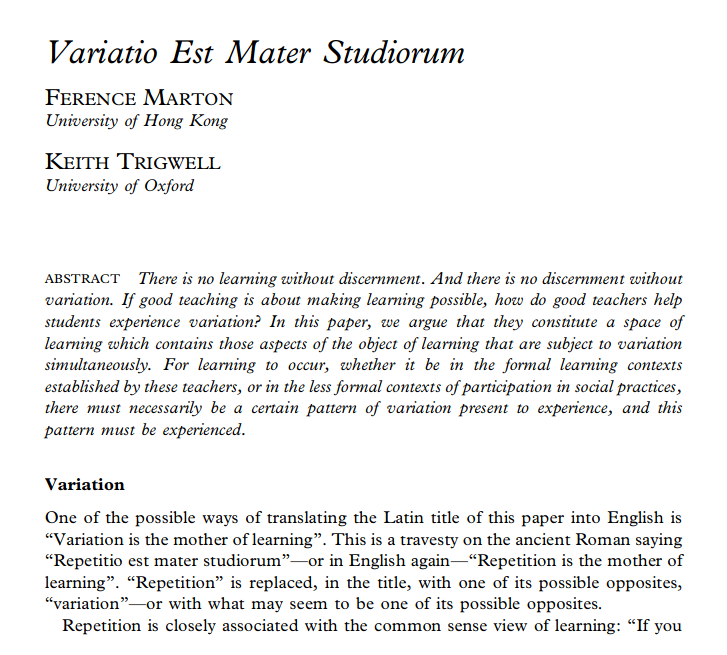
\includegraphics[width=0.8\columnwidth]{figs/variatio-mater-studiorum.png}
        \end{column}
        \begin{column}{0.4\columnwidth}
          
\includegraphics[height=0.55\textheight]{figs/NCOL.jpg}
        \end{column}
      \end{columns}
  \end{remark}
\end{frame}

The design of the course is based on the variation theory of learning~\cite[see 
\eg][]{NecessaryConditionsOfLearning}.
The goal of the theory is to achieve learning that prepares for unknown 
situations.
It aims for deep learning (as opposed to surface learning, 
\cf~\cite{DeepSurfaceLearning}).
This fits very well with our learning outcomes (\cref{LearningOutcomes}).
In fact, \textcite{NecessaryConditionsOfLearning} makes a point that learning 
(according to this theory), is in fact very aligned with science and research.
However, variation theory, according to me, tells us more than the scientific 
method traditionally does; it tells us about the preconditions to scientific 
discovery.

But what does this mean for the course concretely?
Well, in a sense, we could say that the teaching will treat some situations and 
the assessment will treat something \enquote{completely different}.
Of course, there is something in common, namely the essence of the course.
But the purpose of the assessment is to test if the student can use what 
they've learned from the teaching to handle this unknown situation---because 
that's what the thesis and the rest of their careers are about.
Now this also means that if a student adopts the approach of opening the 
assignments and then try to find the correct answers in the teaching material, 
that student will be very disappointed in the course.

In essence, we will look at problems and work out suitable methods to answer 
questions about the problem at hand.
(This is the pattern of variation called contrast, in terms of 
\cite{NecessaryConditionsOfLearning}, and focuses on \ref{LOrelate}, it's the 
first and crucial step of learning.)
Then we'll dive into each method to explore what kinds of questions it can help 
answer.
(This is the pattern of variation called generalization, in terms of 
\cite{NecessaryConditionsOfLearning}, and focuses on \ref{LOevaluate}.
Coincidentally, this pattern corresponds to what is called the scientific 
method.)
Finally, we will combine the methods to answer more complex questions.
(This is the variation of fusion, in terms of 
\cite{NecessaryConditionsOfLearning}, and focuses on \ref{LOapply}.)
The assessment will then be a new problem where the students must combine the 
methods to answer more complex questions on their own.

For the remaining learning objectives, \ref{LOplan} and \ref{LOcomm}, we will 
use the students' own works as learning material.
The idea is as follows:
The students will review each others' works, so this concerns \ref{LOcomm}.
If the work is about arguing why a method answers a particular research 
question, then another student's solution will provide a contrasting 
perspective to one's own.
Even if the choice of method is the same, the phrasing of the arguments 
provides contrast to one's own arguments and phrasing thereof.

We allow for \ref{LOplan} by giving the teaching material, assignments and 
their deadlines for participating in seminars in advance.
Since the course runs in every period, it's up to the student to make a plan 
for when to complete the assignments and participate in the seminars.
It's fine if a plan needs adapting, life happens; the important thing is that 
the students learn to deal with it.
The assessment of this learning outcome consists of evaluating the plan, how it 
turned out and what the student learned.


